\documentclass{amsart}

%%%%%%%%%%%%%%%

\usepackage[utf8]{inputenc}
% \usepackage[spanish]{babel}
% \usepackage[top=1in, bottom=1in, left=1.2in, right=1.2in]{geometry}
\usepackage{amssymb}
\usepackage{amsmath}
\usepackage{amsfonts}
\usepackage{amsthm}
\usepackage{wasysym}
\usepackage{enumitem}
\usepackage{graphicx}
\usepackage{listings}
\usepackage{xcolor}
\usepackage{tikz}

% sets
\newcommand{\NN}{\mathbf{N}}
\newcommand{\ZZ}{\mathbf{Z}}
\newcommand{\QQ}{\mathbf{Q}}
\newcommand{\RR}{\mathbf{R}}
\newcommand{\Zpos}{\ZZ^{+}}
\newcommand{\Rpos}{\RR^{+}}

% brackets
\newcommand{\la}{\langle}
\newcommand{\ra}{\rangle}

% formal statements
\newtheorem{prop}{Proposition}

\theoremstyle{plain}
\newtheorem{clm}{Claim}

\theoremstyle{definition}
\newtheorem{defn}{Definition}

\newtheorem{exl}{Example}

\theoremstyle{remark}
\newtheorem{rmk}{Remark}

% vulgar display of code

\lstdefinestyle{astyle}{
	commentstyle=\color{blue},
	keywordstyle=\color{purple},
	numberstyle=\tiny\color{gray},
	stringstyle=\color{green},
	basicstyle=\ttfamily\footnotesize,
	tabsize=2
}

\lstset{style=astyle}


\title{Coproduct of Operads}
\author{Daniel R. Barrero R.}
\date{\today}

\begin{document}

% -	C.f. work log of June 28	- %

\maketitle

\section{Trees}

%
% Trees for Baez' operads
%

\begin{defn}\label{def-tree}
	An $n-$\emph{tree} is the data $(V, E, s, t)$ where
	\begin{itemize}
		\item $V$ is a finite set of \emph{vertices},
		\item $E$ is a finite set of \emph{edges},
		\item $s : E \to V \cup [1..n]$ is the
			\emph{source map}\footnote{Here we're using the
			comprehension $[a..b] :=
			\{t \in \ZZ \ | \ a \leq t \leq b\}$}, and
		\item $t : E \to V \cup \{0\}$ is the \emph{target map}.
	\end{itemize}
	This data is restricted to satisfy the following conditions:
	\begin{enumerate}
		\item It defines a graph-theoretic tree with vertices
			$V \cup [0..n]$ and edges $E$.
		\item There is exactly one $e \in E$ such that $t(e) = 0$.
	\end{enumerate}
	We use $u \to^{e} v$ to denote\footnote{Since the vertices and
	edges form a tree,  specifying the edge is redundant. We will keep
	this definition for the time being in order to fluidly converse
	with the authors.} that $e \in E$ has source $u$ and target $v$.
\end{defn}

\begin{defn}\label{tree-iso}
	We say that the trees $(V,E,s,t)$ and $(V',E',s',t)$ are
	\emph{isomorphic} if there exist bijections $F_0 : V \cup [0..n]
	\to V' \cup [0..n]$ and $F_1 : E \to E'$ such that
	\begin{eqnarray}
		F_0s= s'F_1\\
		F_0t= t'F_1\\
		F_0\ \text{restricted to } [0..n]\ \text{is a bijection.}
	\end{eqnarray}
	In other words, two $n-$trees are isomorphic if they are equal
	modulo renaming of their vertices and edges.
\end{defn}

\begin{exl}
	The following trees are isomorphic

	\begin{tikzpicture}
		\node (A) at (1, 0) {};
		\node[minimum size=0mm, inner sep=0pt] (B) at (1, 1) {};
		\node[minimum size=0mm, inner sep=0pt] (C) at (0.5, 1.5) {};
		\node (D) at (0, 2) {1}; \node (E) at (1, 2) {2};
		\node (F) at (2, 2) {3};
		%
		\node (symb) at (2.5, 1) {$\simeq$}; % Equivalence symbol
		%
		\node (A') at (4, 0) {};
		\node[minimum size=0mm, inner sep=0pt] (B') at (4, 1) {};
		\node[minimum size=0mm, inner sep=0pt] (C') at (4.5, 1.5) {};
		\node (D') at (3, 2) {3}; \node (E') at (4, 2) {2};
		\node (F') at (5, 2) {1};
		% Drawing the edges
		%% Left tree
		\draw (A) to (B); \draw (B) to (C); \draw (B) to (F);
		\draw (C) to (D); \draw (C) to (E);
		%% Right tree
		\draw (A') to (B'); \draw (B') to (C'); \draw (B') to (D');
		\draw (C') to (E'); \draw (C') to (F');
	\end{tikzpicture}
\end{exl}

%

\begin{exl}
	The following trees are not isomorphic

	\begin{tikzpicture}
		% Picture nodes
		%% Left tree
		\node (N) at (1, 0) {};
		\node[minimum size=0mm, inner sep=0pt] (Ni) at (1, 1) {};
		\node[minimum size=0mm, inner sep=0pt] (Nii) at (0.5, 1.5) {};
		\node (1) at (0, 2) {1};
		\node (2) at (1, 2) {2};
		\node (3) at (2, 2) {3};
		%% Symbol
		\node (symb) at (2.5, 1) {$\not\simeq$};
		%% Right tree
		\node (N') at (4, 0) {};
		\node[minimum size=0mm, inner sep=0pt] (N'i) at (4, 1) {};
		\node[minimum size=0mm, inner sep=0pt] (N'ii) at (3.5, 1.5) {};
		\node (1') at (3, 2) {1};
		\node (2') at (5, 2) {2};
		\node (3') at (4, 2) {3};
		% Picture arcs
		%% Left tree edges
		\draw (N) to (Ni);
		\draw (Ni) to (Nii);
		\draw (Ni) to (3);
		\draw (Nii) to (1);
		\draw (Nii) to (2);
		%% Right tree edges
		\draw (N') to (N'i);
		\draw (N'i) to (N'ii);
		\draw (N'i) to (2');
		\draw (N'ii) to (1');
		\draw (N'ii) to (3');
	\end{tikzpicture}

	For instance because the lengths of the paths from the root to node 3 are
	different.\footnote{The reader can check that path length is
		isomorphism-invariant.}
\end{exl}

\begin{defn}\label{tree-v}
	This is some vocabulary associated with $n-$trees:
	\begin{itemize}
		\item The \emph{children} of the vertex $v$ are the
			elements of $t^{-1} \ \{ v \}$, and the cardinality
			of this set is the \emph{arity} of $v$.
		\item A 0-ary vertex is called a \emph{terminus}.
		\item A tree with one vertex is called a \emph{corolla}.
		\item The edge whose target is the root, and the edges
			whose sources are the leaves, are called
			\emph{external edges}, and the remaining edges are
			the \emph{internal edges}.
	\end{itemize}
\end{defn}

We now define grafting/partial composition for trees.
\begin{defn}
	Let $f= (m, V', E', s', t')$ and $g= (n, V, E, s, t)$ be trees and let 
	$i \in [1..m]$. The \emph{grafting of $g$ onto $f$ along $i$} is the tree

	\begin{equation*}
		f \circ_i g= (n+m-1, \tilde{V}, \tilde{E}, \tilde{s}, \tilde{t})
	\end{equation*} where

	\setcounter{equation}{0}
	\begin{eqnarray}
		\tilde{V}= V' \cup V,\\
		\tilde{E}= (E' \cup E \cup \{x\}) - \{e'_i, e_0\}
	\end{eqnarray} and

	\begin{displaymath}
		\tilde{s}(e)=
		\begin{cases}
			s'(e)\ \text{if}\ e \in E'\ \text{and}\ s'(e) \in V',\\
			s'(e)\ \text{if}\ e \in E'\ \text{and}\ s'(e) \in [0..i-1],\\
			s'(e) + n-1\ \text{if}\ e \in E'\ \text{and}\ s'(e) \in [i+1..m],\\
			s(e_0)\ \text{if}\ e = x,\\
			s(e)\ \text{if}\ e \in E\ \text{and}\ s(e) \in V,\\
			s(e) + i-1\ \text{if}\ e \in E\ \text{and}\ s(e) \in [1..n]
		\end{cases}
	\end{displaymath}

	\begin{displaymath}
		\tilde{t}(e)=
		\begin{cases}
			t'(e)\ \text{if}\ e \in E',\\
			t(e)\ \text{if}\ e \in E,\\
			t'(e'_i)\ \text{if}\ e = x
		\end{cases}
	\end{displaymath} where $e_0$ is the edge of $g$ with target $0$ and $e'_i$ is the
	edge of $f$ with source $i$.
\end{defn}

**DRAW GRAFTING EXAMPLES HERE**

\bigskip

We now define planar trees.
\begin{defn}[Planar trees]\label{plts}
	A \emph{planar $n-$tree} is an $n-$tree such that each vertex is equipped
	with a linear ordering on the set of its children. An \emph{isomorphism}
	of such trees is one that preserves the linear orderings.
\end{defn}

We now define trees with lengths.
\begin{defn}[Trees with lengths]\label{twl}
	An $n-$tree \emph{with lengths} is the data $(T,l)$ where $T$ is an $n-$tree
	and $l : E \to [0, \infty[$. The \emph{length function} $l$ clearly makes $T$
	into a planar tree.
\end{defn}

\begin{defn}[Phylogenetic trees]\label{phts}
	A \emph{phylogenetic $n-$tree} is an isomorphism class of $n-$trees with lengths satisfying the following conditions:
	\begin{enumerate}
		\item \emph{There are no unary vertices nor termini}, and
		\item \emph{There are no internal edges of length 0}.
	\end{enumerate}
\end{defn}

A drawing:

\begin{center}
	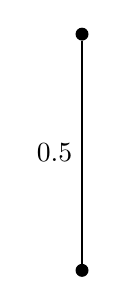
\begin{tikzpicture}[auto]
		\node[circle, draw, fill, inner sep=0pt, minimum size=1.5mm] (1) at (0,0) {};
		\node[circle, draw, fill, inner sep=0pt, minimum size=1.5mm] (2) at (0,3) {};

		\draw (1) to node {0.5} (2);
	\end{tikzpicture}
\end{center}


% green!50!black produces a dark green.

Was it successful?

Now Java code:

\lstinputlisting[language=Java, firstline=1, lastline=4]{inJava.java}

Successful?


% % - Definitions are maybe too conversational.


\section{Free operads}

Let $U : \mathrm{Op} \to \mathrm{Top}^{\NN}$ be the forgetful functor and
let $F$ be its left adjoint. Its existence is a result of Boardman and Vogt
in \cite{bv-hiasots}.

\begin{defn}
	Let $C$ be a collection. A \emph{$C-$labelled planar $n-$tree} is a
	planar $n-$tree such that each vertex with $k$ children is labelled
	by an element of $C_k$.
\end{defn}


	

\section{The construction}

Given two operads $O$ and $O'$, the $F-U$ adjoint pair gives epimorphisms 

\begin{eqnarray}\label{fu-epis}
	\epsilon : FU \ O \to O \\
	\epsilon' : FU \ O' \to O'.
\end{eqnarray}

If the category $\mathrm{Op}$ had coproducts, we would have an operad
epimorphism\footnote{It being an epimorphism is not immediate, but the
property is necessary for the validity of the construction.}

\begin{equation}\label{cpd-epis}
	\epsilon + \epsilon' : (FU \ O) + (FU \ O') \to O + O'.
\end{equation}

Drawing inspiration\footnote{We haven't established nor cited any relevant
categorical properties for operads.} from the fact that left adjoints
preserve colimits \cite{riehl-ctic}, we may define


\begin{equation}\label{fu-coprod}
	(FU \ O) + (FU \ O') \ := \ F \ \left( (U \ O) + (U \ O')
	\right).
\end{equation}

and therefore compute a quotient of $F \ \left( (U \ O) + (U \ O')
\right)$ that is a coproduct of $O$ and $O'$.

\section{Algebras}


In order for $A$ to be an algebra over $O + O'$, it only requires having
algebra structrues over both $O$ and $O'$, with no compatibility conditions
imposed:

\begin{equation}\label{opd-cpd}
		\begin{tikzcd}
			& O + O' \arrow[dd, dashed, "u + v" description] &
					\\
			O \arrow[rd, "u"'] \arrow[ru, "i"] & & O'
				\arrow[ld, "v"] \arrow[lu, "j"'] \\
			& \mathrm{End}(A) &
		\end{tikzcd}
\end{equation}

\section{Comments}

\subsection{} The result by B \& V is that the forgetful functor is
\emph{monadic.}

\subsection{} The full statement that motivates \eqref{fu-coprod} is that
\emph{Right adjoints preserve limits and left adjoints preserve colimits.}
It can be found in \cite{riehl-ctic}.

\subsection{} The definition \eqref{fu-coprod} suggests that
\emph{``at the $FU-$level coproducts are trivially definied.''}

\subsection{} Justify that $\epsilon + \epsilon'$ in \eqref{cpd-epis} is
an epimorphism.

\subsection{} The number of edges of a tree given by definition
\ref{def-tree} is probably

$$
(\# \ V) + n,
$$

where $n$ is the number of leaves.

\subsection{Yoneda's lemma} I must write down this simple but important
fact at some point.

\subsection{General products and coproducts}

\begin{defn}\label{prod-def}
	Let $X$ and $Y$ be objects of the category $\mathcal{C}$. Their
	\emph{product}, if it exists, is the data $(X \times Y, p, q)$
	uniquely determined by the property that for any object $Z$ of
	$\mathcal{C}$ and maps $f : Z \to X$ and $g : Z \to Y$, the
	following diagram commutes:
	\begin{equation}\label{prod-cd}
		\begin{tikzcd}
			& X \times Y \arrow[ld, "p"'] \arrow[rd, "q"] & \\
			  X &            & Y \\
			  & Z \arrow[lu, "f"] \arrow[ru, "g"']
			      \arrow[uu, dashed, "f \times g" description] & 
		\end{tikzcd}
	\end{equation}
\end{defn}

We obtain the definition of coproduct by inverting the directions of the
arrows in definition \ref{prod-def}:

\begin{defn}\label{coprod-def}
	The \emph{coproduct} of $X$ and $Y$, if it exists, is the data
	$(X + Y, i, j)$ uniquely determined by the property that for any
	object $Z$ and maps $u : X \to Z$ and $v : Y \to Z$, the following
	diagram commutes:
	\begin{equation}\label{coprod-cd}
		\begin{tikzcd}
			& X + Y \arrow[dd, dashed, "u + v" description] &
					\\
			X \arrow[rd, "u"'] \arrow[ru, "i"] & & Y
				\arrow[ld, "v"] \arrow[lu, "j"'] \\
			& Z &
		\end{tikzcd}
	\end{equation}
\end{defn}

\bibliographystyle{acm}
\bibliography{refs}

\end{document}
